\subsubsection{Các màn hình dành cho Admin}
\label{sec:admin-implementation}

Kênh Admin tập trung các công việc xét duyệt, quản lý quyền, xử lý báo cáo và tra cứu nhật ký. Màn hình tổng quan cung cấp lối vào từng nhóm; các hàng đợi được trình bày bằng thẻ hồ sơ hoặc tin đăng. AdminViewModel giữ nhóm đang chọn và trạng thái request, còn AdminRepository truy vấn theo loại đối tượng. Bộ đếm hàng đợi được tính từ dữ liệu vừa tải trong giới hạn truy vấn, không phải số liệu tổng hợp toàn hệ thống.

Hàng đợi Host lấy những đơn đang PENDING từ \texttt{hostApplications}. Mỗi thẻ gồm thông tin người nộp, nội dung hồ sơ và tệp giấy tờ DEMO. Giao diện yêu cầu mở các tệp minh chứng trước khi gửi quyết định chấp thuận. Trong transaction xét duyệt, Repository đọc lại quyền Admin, trạng thái đơn và hồ sơ người nộp. Khi chấp thuận, trạng thái đơn, quyền HOST trong \texttt{users}, bản chiếu \texttt{publicHosts} và audit được cập nhật cùng thao tác. Khi từ chối, lý do được lưu để người nộp có thể bổ sung hồ sơ.

\IfFileExists{Resources/chapter5/admin-overview.png}{%
Màn hình tổng quan trong Hình~\ref{fig:admin-overview-review}(a) tổ chức các lối vào xét duyệt, quản lý, báo cáo và nhật ký. Khi chọn xét duyệt không gian, Admin nhận danh sách phòng PENDING\_REVIEW như Hình~\ref{fig:admin-overview-review}(b). Mỗi thẻ có ảnh, thông tin tóm tắt và nút mở nội dung đầy đủ trước khi duyệt hoặc từ chối. Repository kiểm lại chủ sở hữu và tòa nhà trước khi ghi quyết định; xét duyệt tin đăng độc lập với cấp quyền Host.
\begin{figure}[H]
\centering
\begin{minipage}[t]{0.40\linewidth}\centering
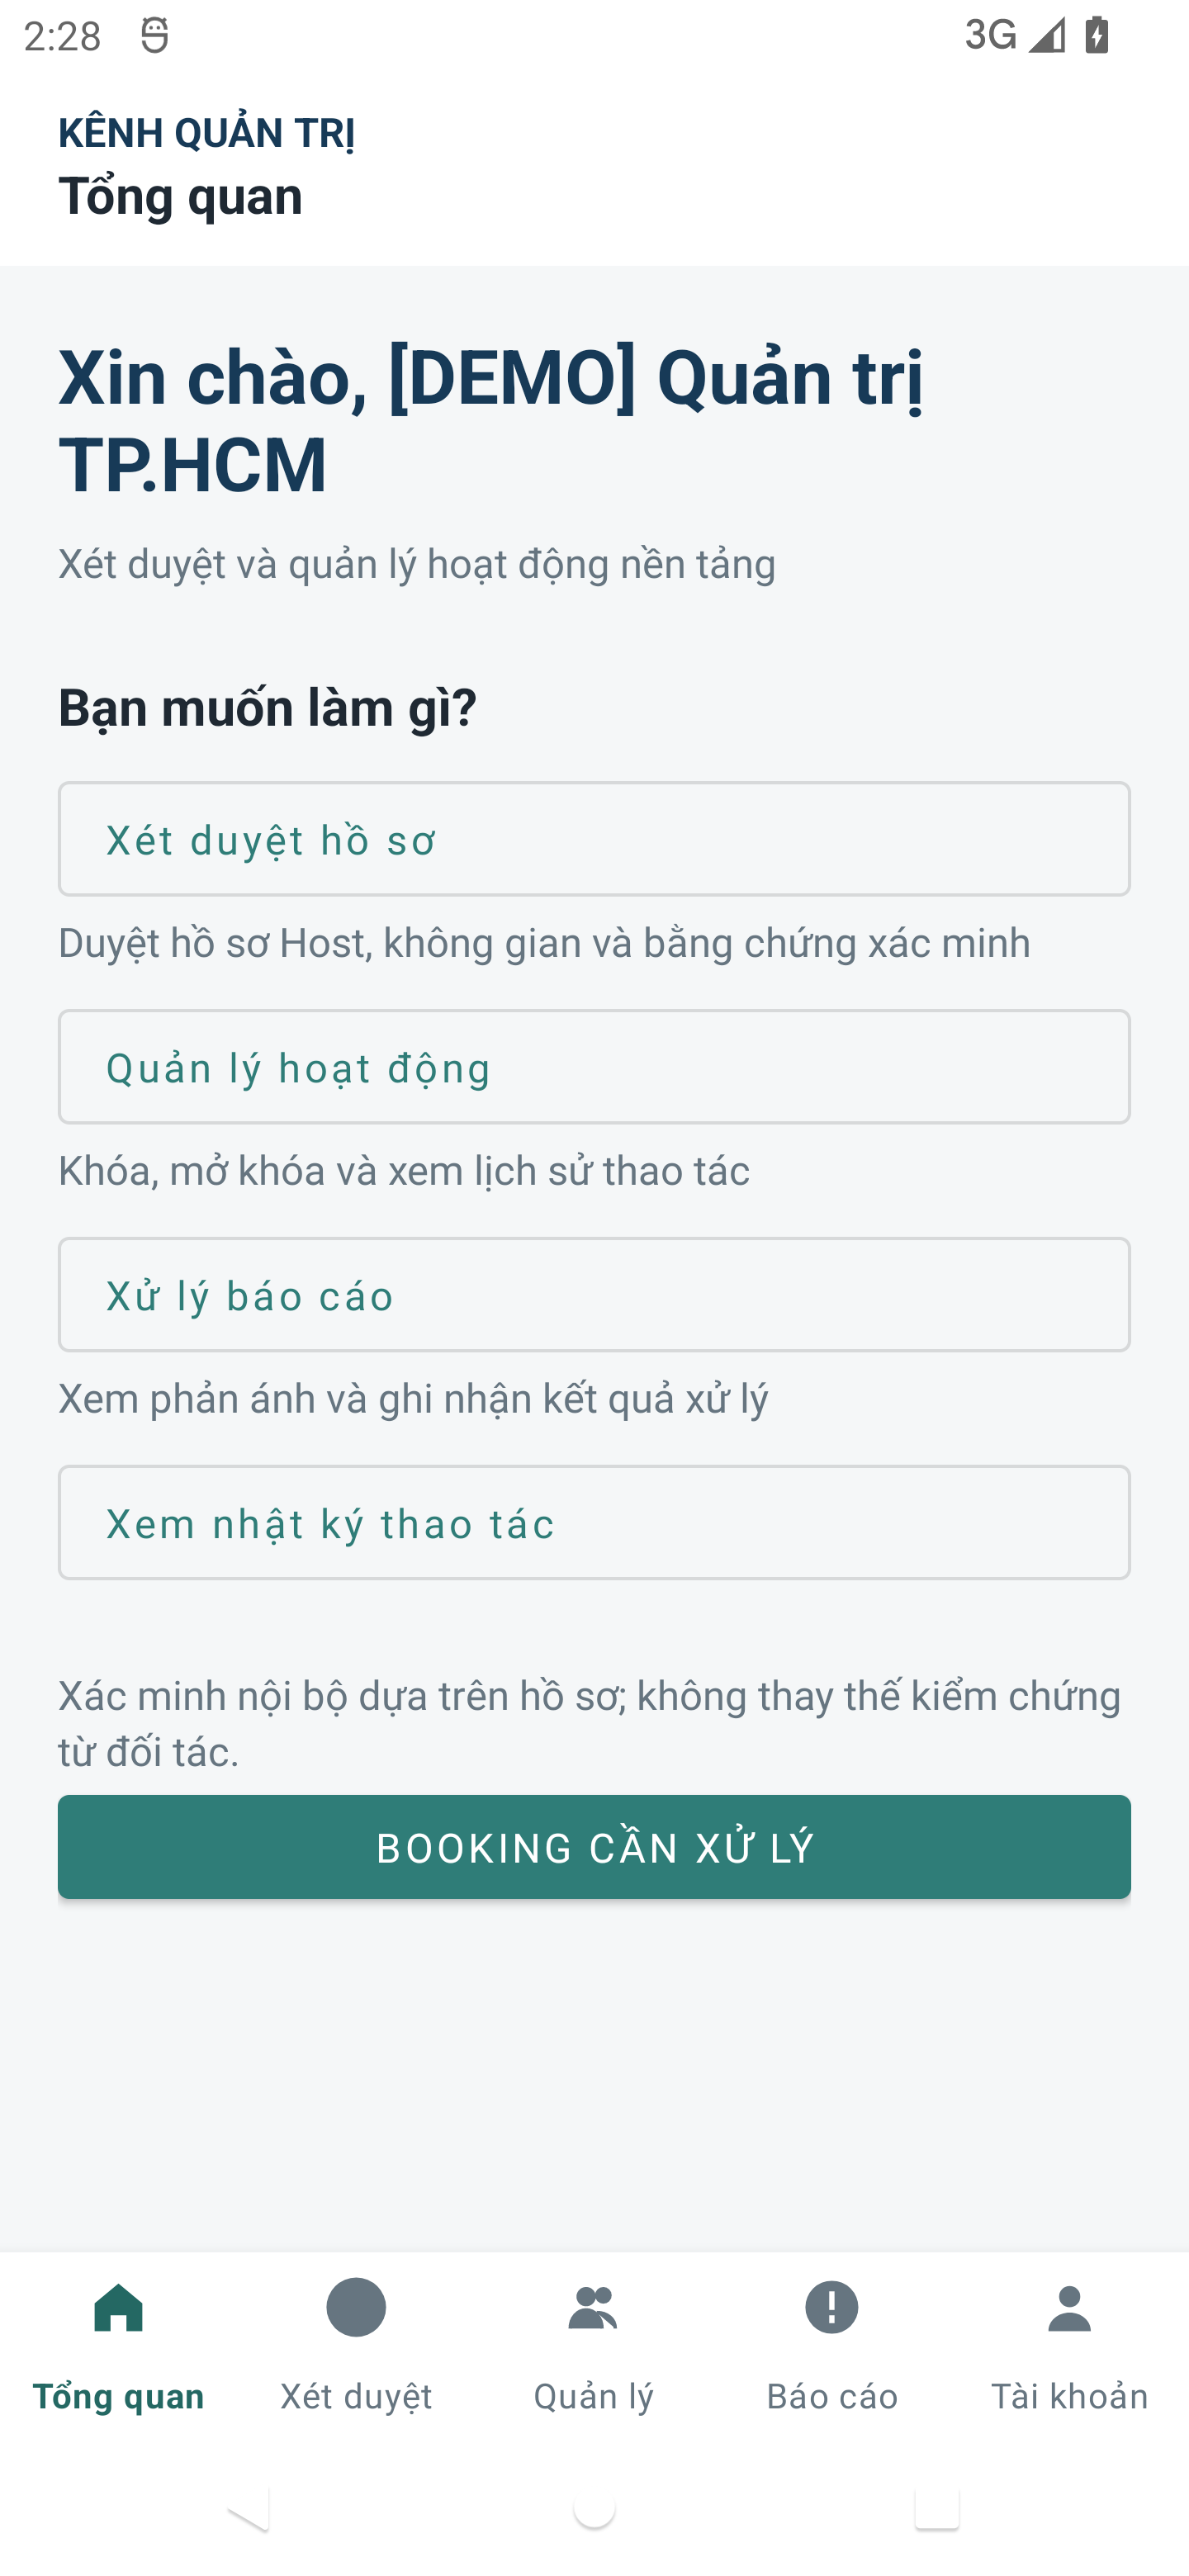
\includegraphics[width=\linewidth]{chapter5/admin-overview.png}\\[-1mm]
{\small (a) Tổng quan quản trị}
\end{minipage}\hspace{0.05\linewidth}%
\begin{minipage}[t]{0.40\linewidth}\centering
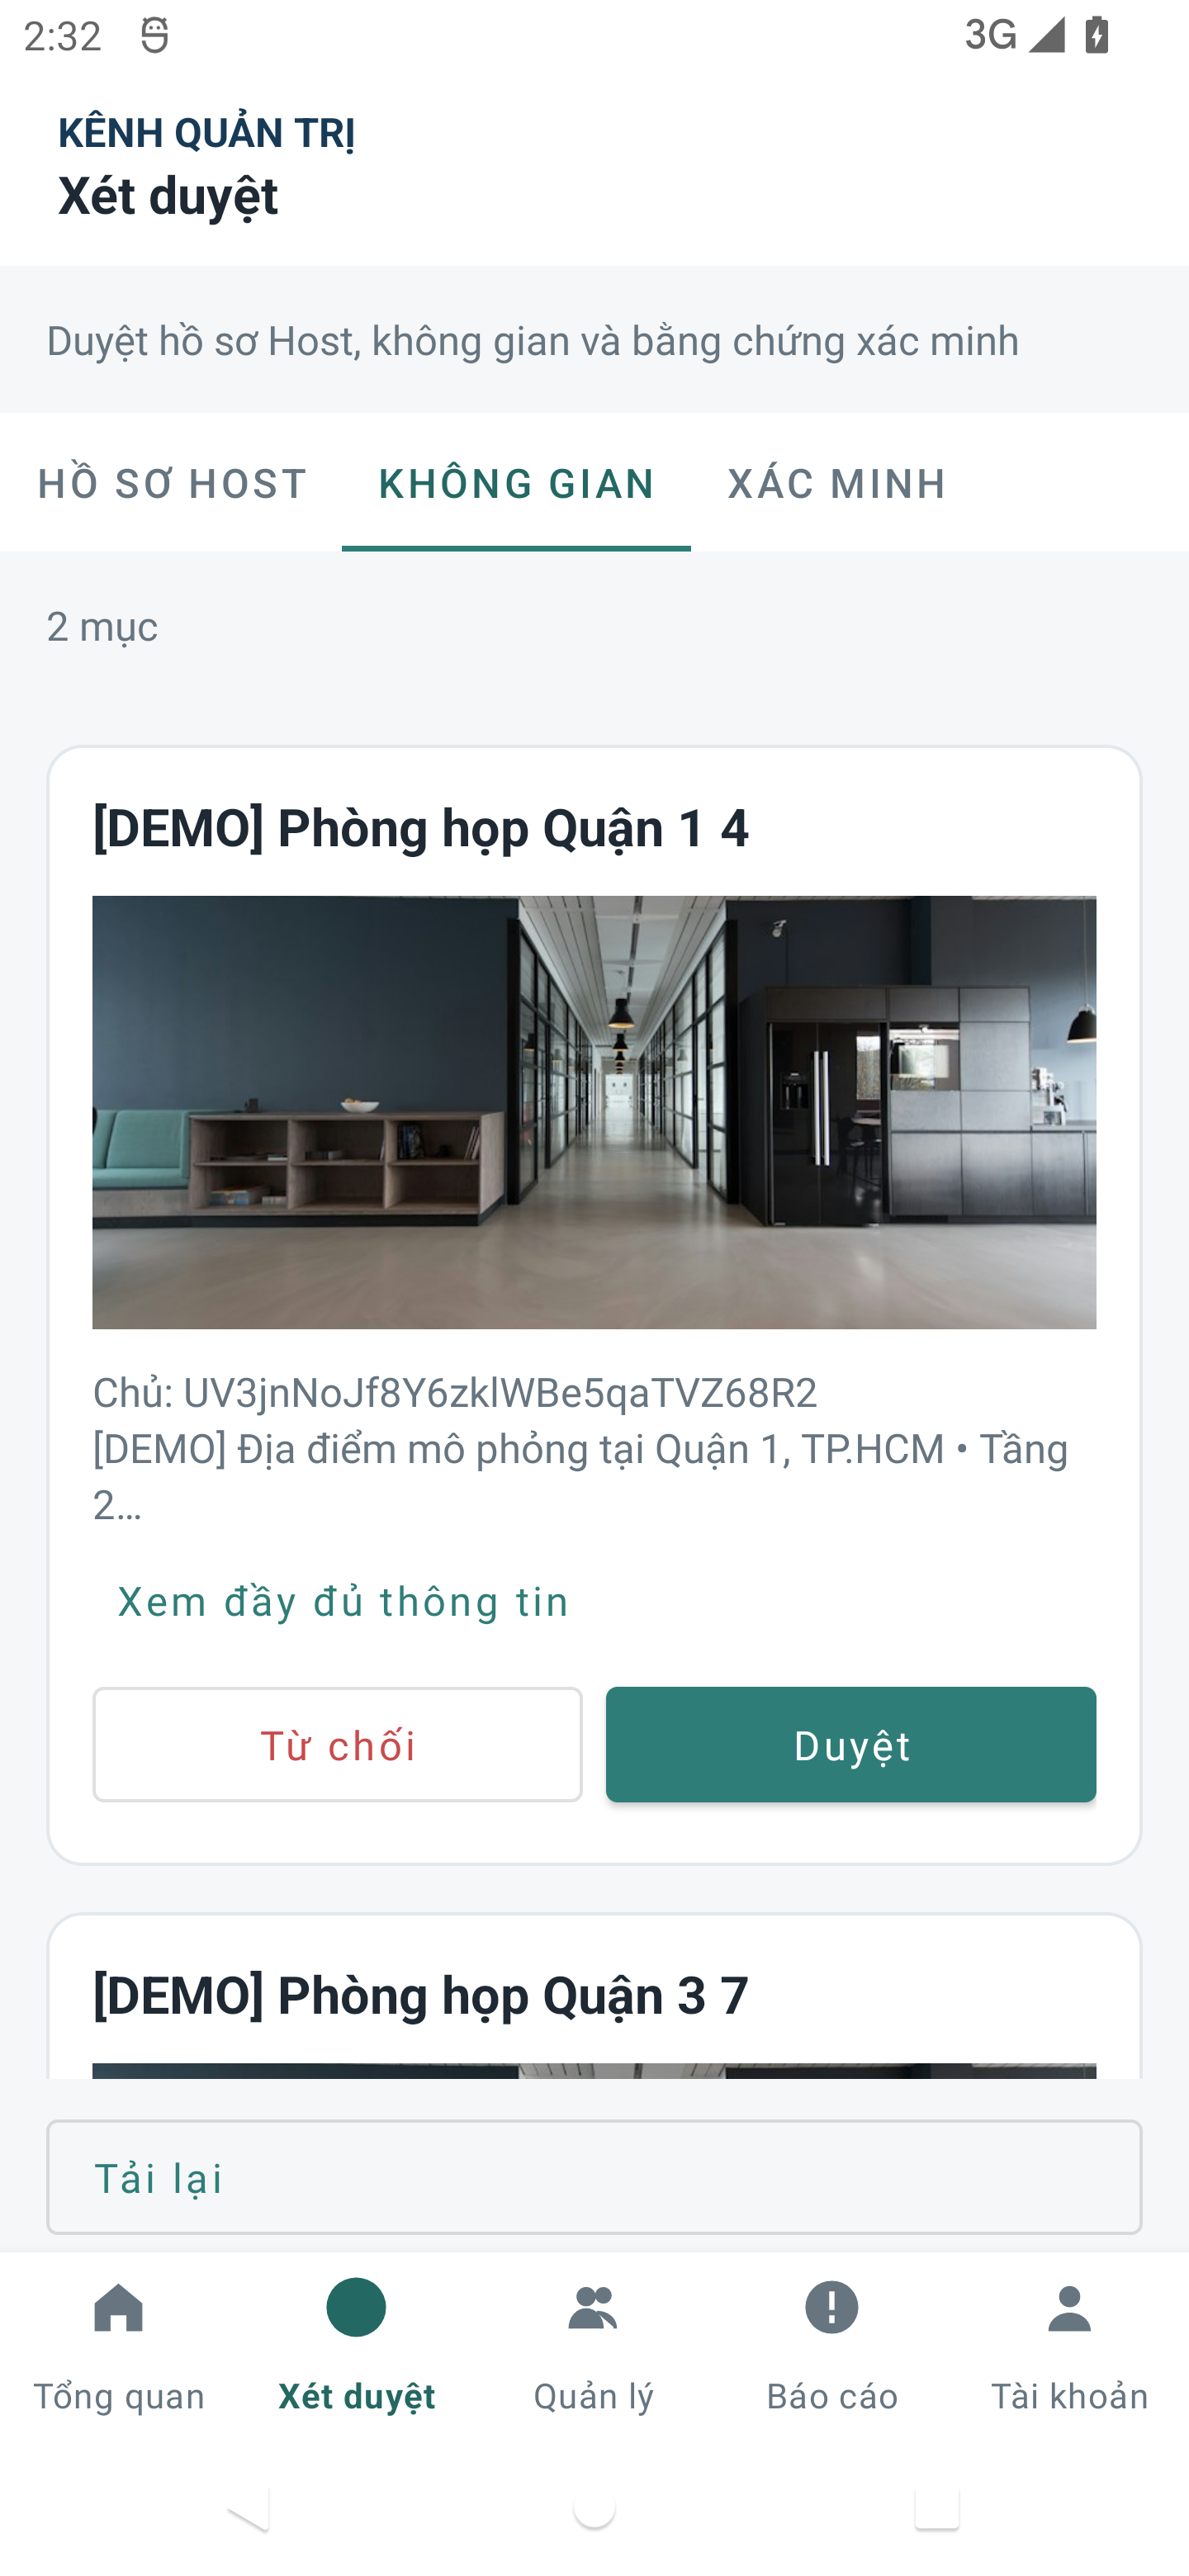
\includegraphics[width=\linewidth]{chapter5/admin-room-review.png}\\[-1mm]
{\small (b) Hàng đợi xét duyệt phòng}
\end{minipage}
\caption{Các màn hình tổng quan và xét duyệt tin đăng của Admin}
\label{fig:admin-overview-review}
\end{figure}}{}

Minh chứng vị trí và hình ảnh được đọc từ \texttt{propertyVerifications}, phân biệt với đơn xin quyền Host. Admin mở tệp ảnh hoặc PDF trong màn xem minh chứng, sau đó gửi kết quả xét duyệt cùng ghi chú. Repository ghi người xử lý, thời điểm và phương thức ADMIN\_REVIEWED; thông tin xác minh liên quan được cập nhật theo đối tượng phòng hoặc tòa nhà. Quy trình xác minh được thực hiện thủ công trên minh chứng DEMO, chưa có đối tác xác thực tự động.

Nhóm quản lý cho phép khóa hoặc mở khóa Host, đình chỉ hoặc gỡ đình chỉ phòng. Trạng thái tài khoản được đồng bộ với bản chiếu Host công khai; các quyền nhận đặt mới và thao tác nghiệp vụ được kiểm lại khi sử dụng. Lịch sử booking không bị xóa khi tài khoản bị khóa. Với báo cáo vi phạm, Admin đọc nội dung, phản hồi của Host và booking liên quan, rồi nhập kết luận. Kết quả được lưu thành RESOLVED hoặc DISMISSED; hành động xử lý có thể là ghi kết luận, đình chỉ phòng hoặc khóa Host.

Các booking cần can thiệp được mở ở màn hình riêng trong Hình~\ref{fig:admin-reports-bookings}. Admin xử lý từng trường hợp, không hủy đồng loạt theo trạng thái Host. Những thao tác như hủy booking chưa check-in của Host bị khóa, kết thúc lượt đang sử dụng do sự cố hoặc xác minh lại việc sử dụng đều yêu cầu căn cứ phù hợp và lý do. BookingRepository kiểm quyền và trạng thái hiện tại, cập nhật lịch khi cần nhả giữ chỗ, đồng thời ghi audit. Việc khép vụ việc không được tự đổi số tiền thành đã thu hoặc đã hoàn.

\IfFileExists{Resources/chapter5/admin-reports.png}{%
Hình~\ref{fig:admin-reports-bookings}(a) trình bày các báo cáo đang chờ xử lý. Admin mở nội dung đầy đủ rồi chọn bỏ qua hoặc ghi nhận kết quả, kèm kết luận và hành động phù hợp. Màn booking ở Hình~\ref{fig:admin-reports-bookings}(b) hiển thị mã đặt chỗ, Host, kỳ thuê và trạng thái của từng lượt. Các thao tác can thiệp được áp dụng cho từng booking sau khi kiểm tra điều kiện, giữ lại lịch sử và lý do xử lý.
\begin{figure}[H]
\centering
\begin{minipage}[t]{0.40\linewidth}\centering
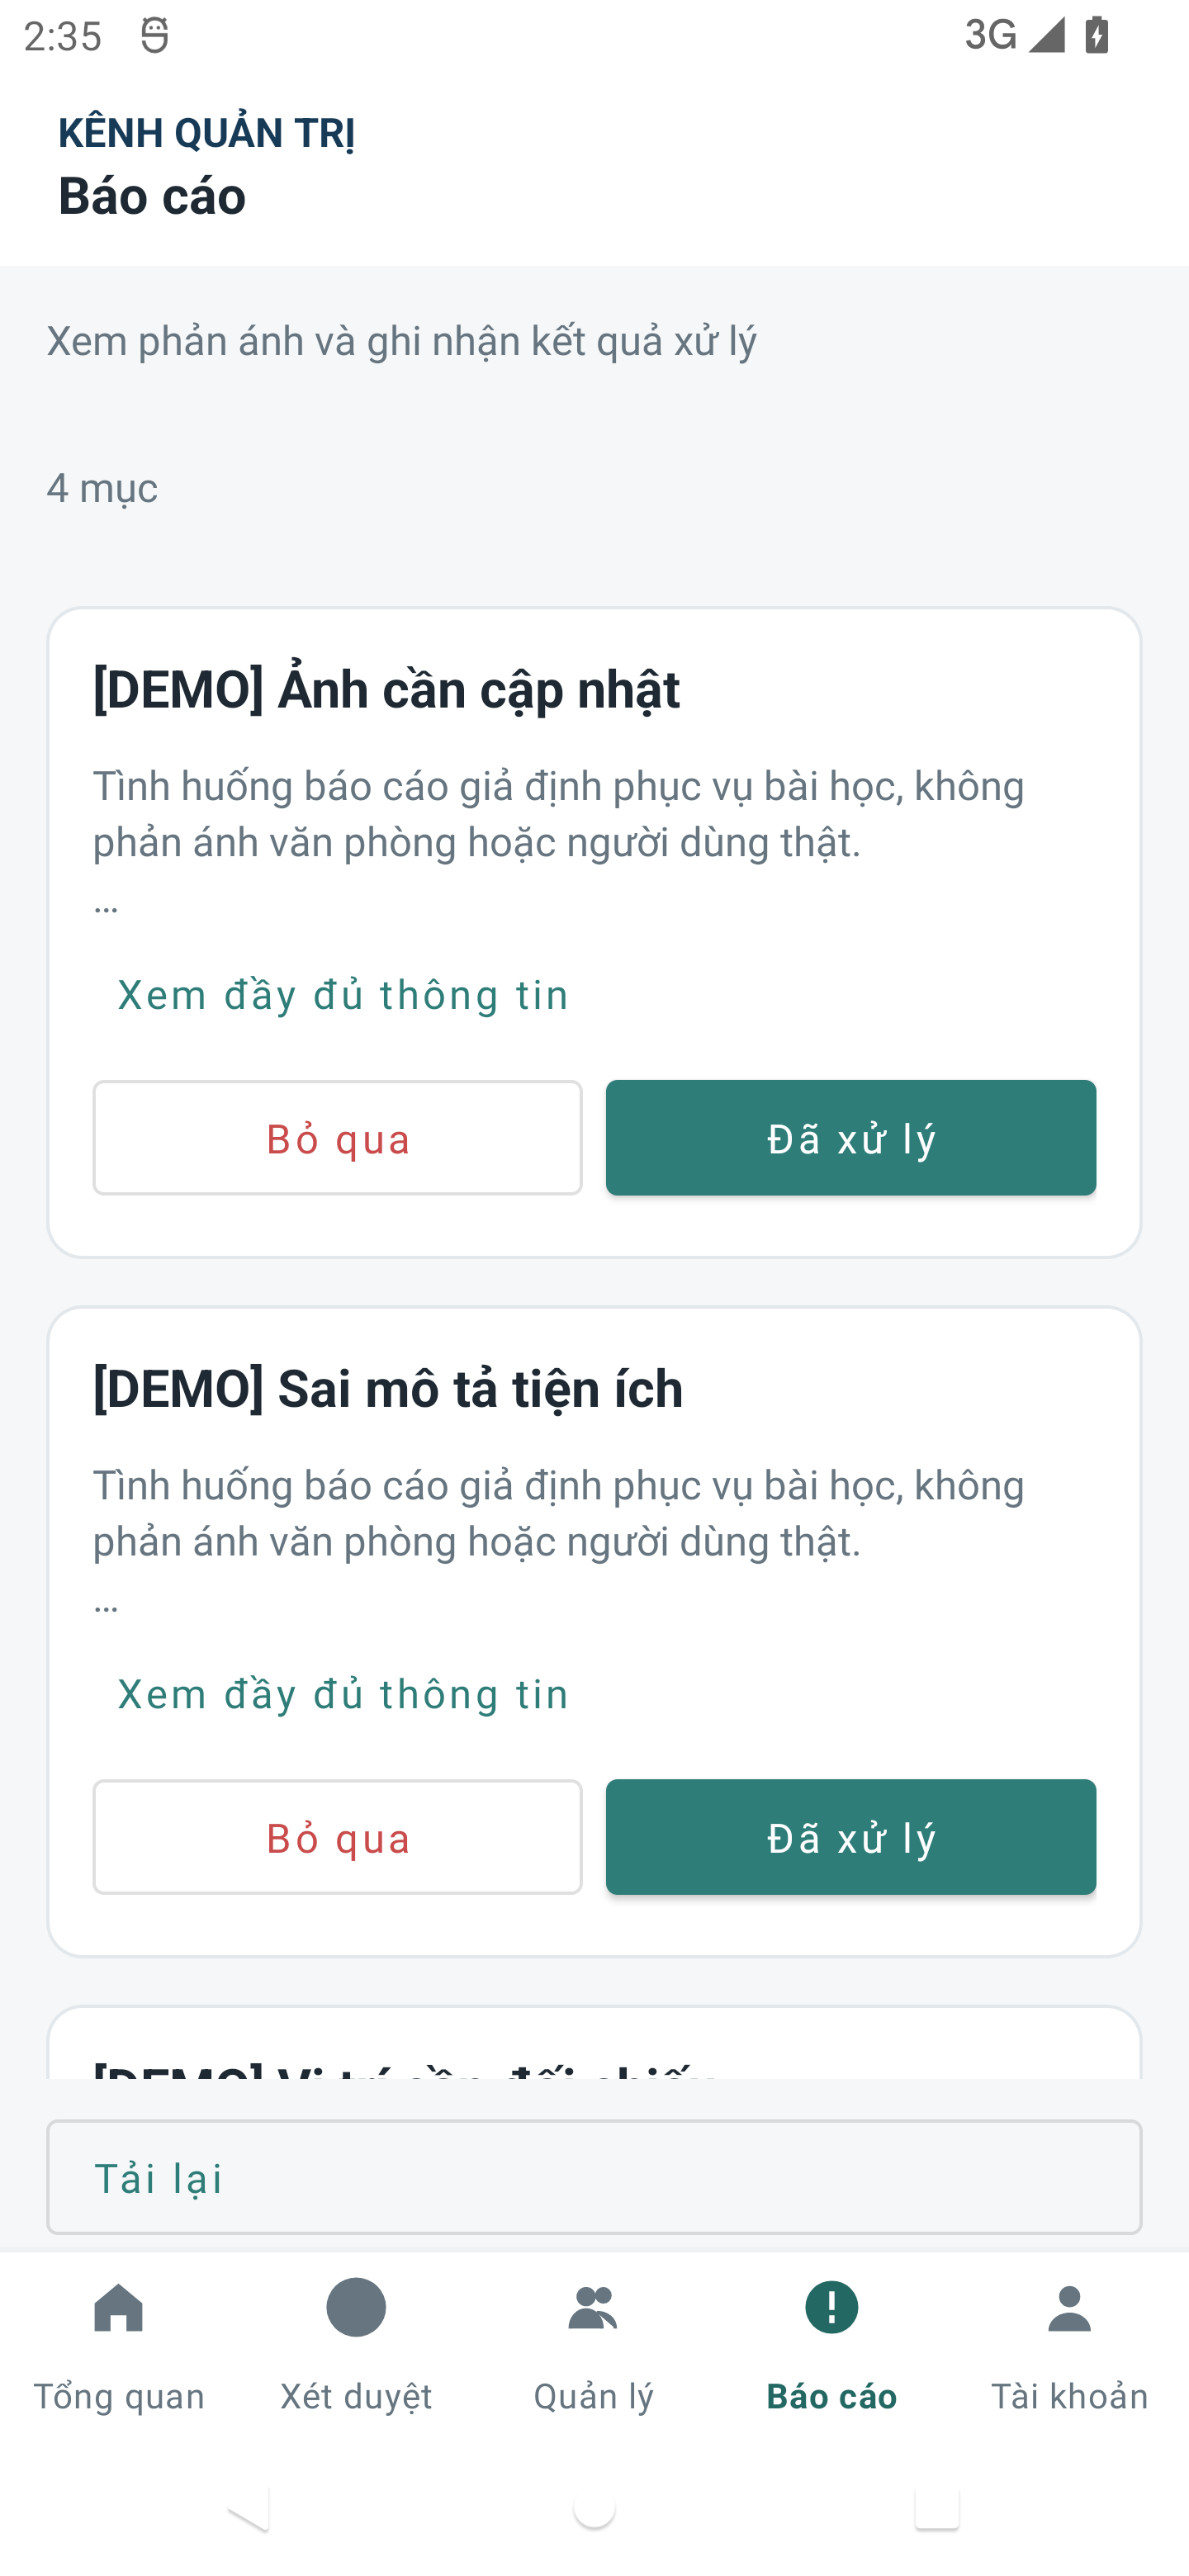
\includegraphics[width=\linewidth]{chapter5/admin-reports.png}\\[-1mm]
{\small (a) Báo cáo cần xử lý}
\end{minipage}\hspace{0.05\linewidth}%
\begin{minipage}[t]{0.40\linewidth}\centering
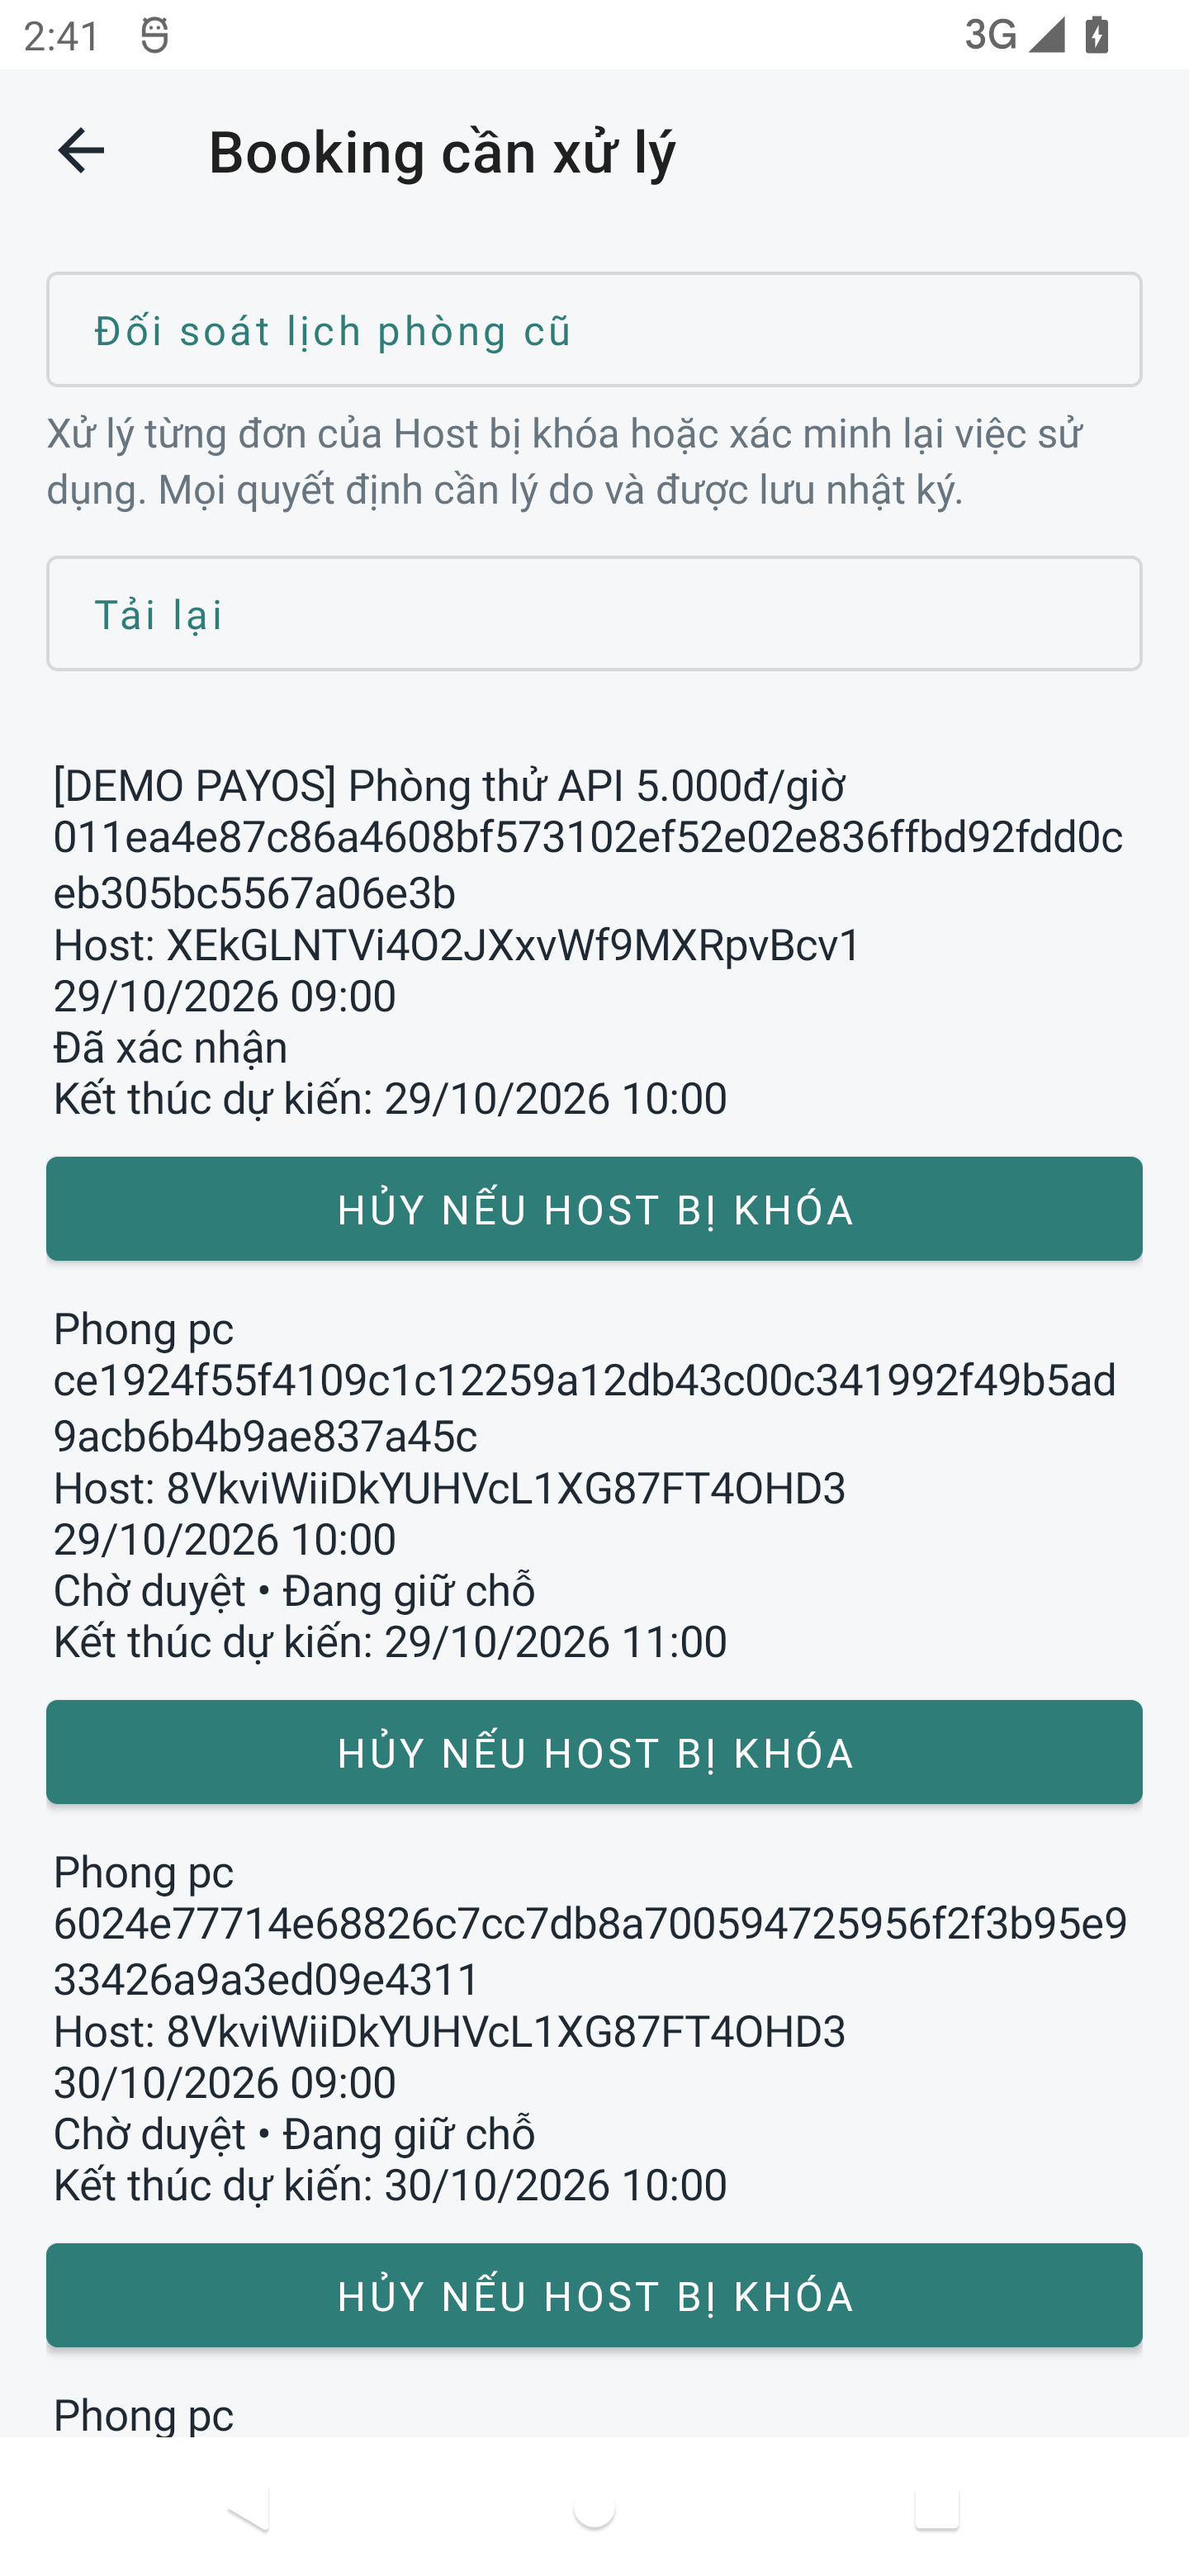
\includegraphics[width=\linewidth]{chapter5/admin-booking-cases.png}\\[-1mm]
{\small (b) Can thiệp từng booking}
\end{minipage}
\caption{Giao diện xử lý báo cáo và booking ngoại lệ}
\label{fig:admin-reports-bookings}
\end{figure}}{}

Màn đối soát lịch kiểm tra số booking còn giữ chỗ của một phòng và các khóa lịch tương ứng trước khi cập nhật bộ đếm. Chức năng này phục vụ trường hợp dữ liệu cũ cần đối chiếu, không tạo thêm phòng hoặc thay đổi hình thức thuê. Nhóm nhật ký đọc \texttt{auditLogs} để hiển thị người thực hiện, đối tượng, hành động và lý do theo thời gian. Hình~\ref{fig:admin-application-evidence} và Hình~\ref{fig:admin-host-audit} bổ sung các hàng đợi xét duyệt và dấu vết xử lý tương ứng.

\IfFileExists{Resources/chapter5/admin-applications.png}{%
Hàng đợi trong Hình~\ref{fig:admin-application-evidence}(a) cung cấp tên, thông tin liên hệ và mô tả hồ sơ xin quyền Host. Admin mở nội dung đầy đủ và tệp giấy tờ trước khi quyết định cấp quyền. Hình~\ref{fig:admin-application-evidence}(b) là hàng đợi minh chứng vị trí và ảnh, hiển thị phòng hoặc tòa nhà cần đối chiếu. Hai hàng đợi phục vụ hai quyết định độc lập: cấp quyền Host và xét duyệt minh chứng không gian.
\begin{figure}[H]
\centering
\begin{minipage}[t]{0.40\linewidth}\centering
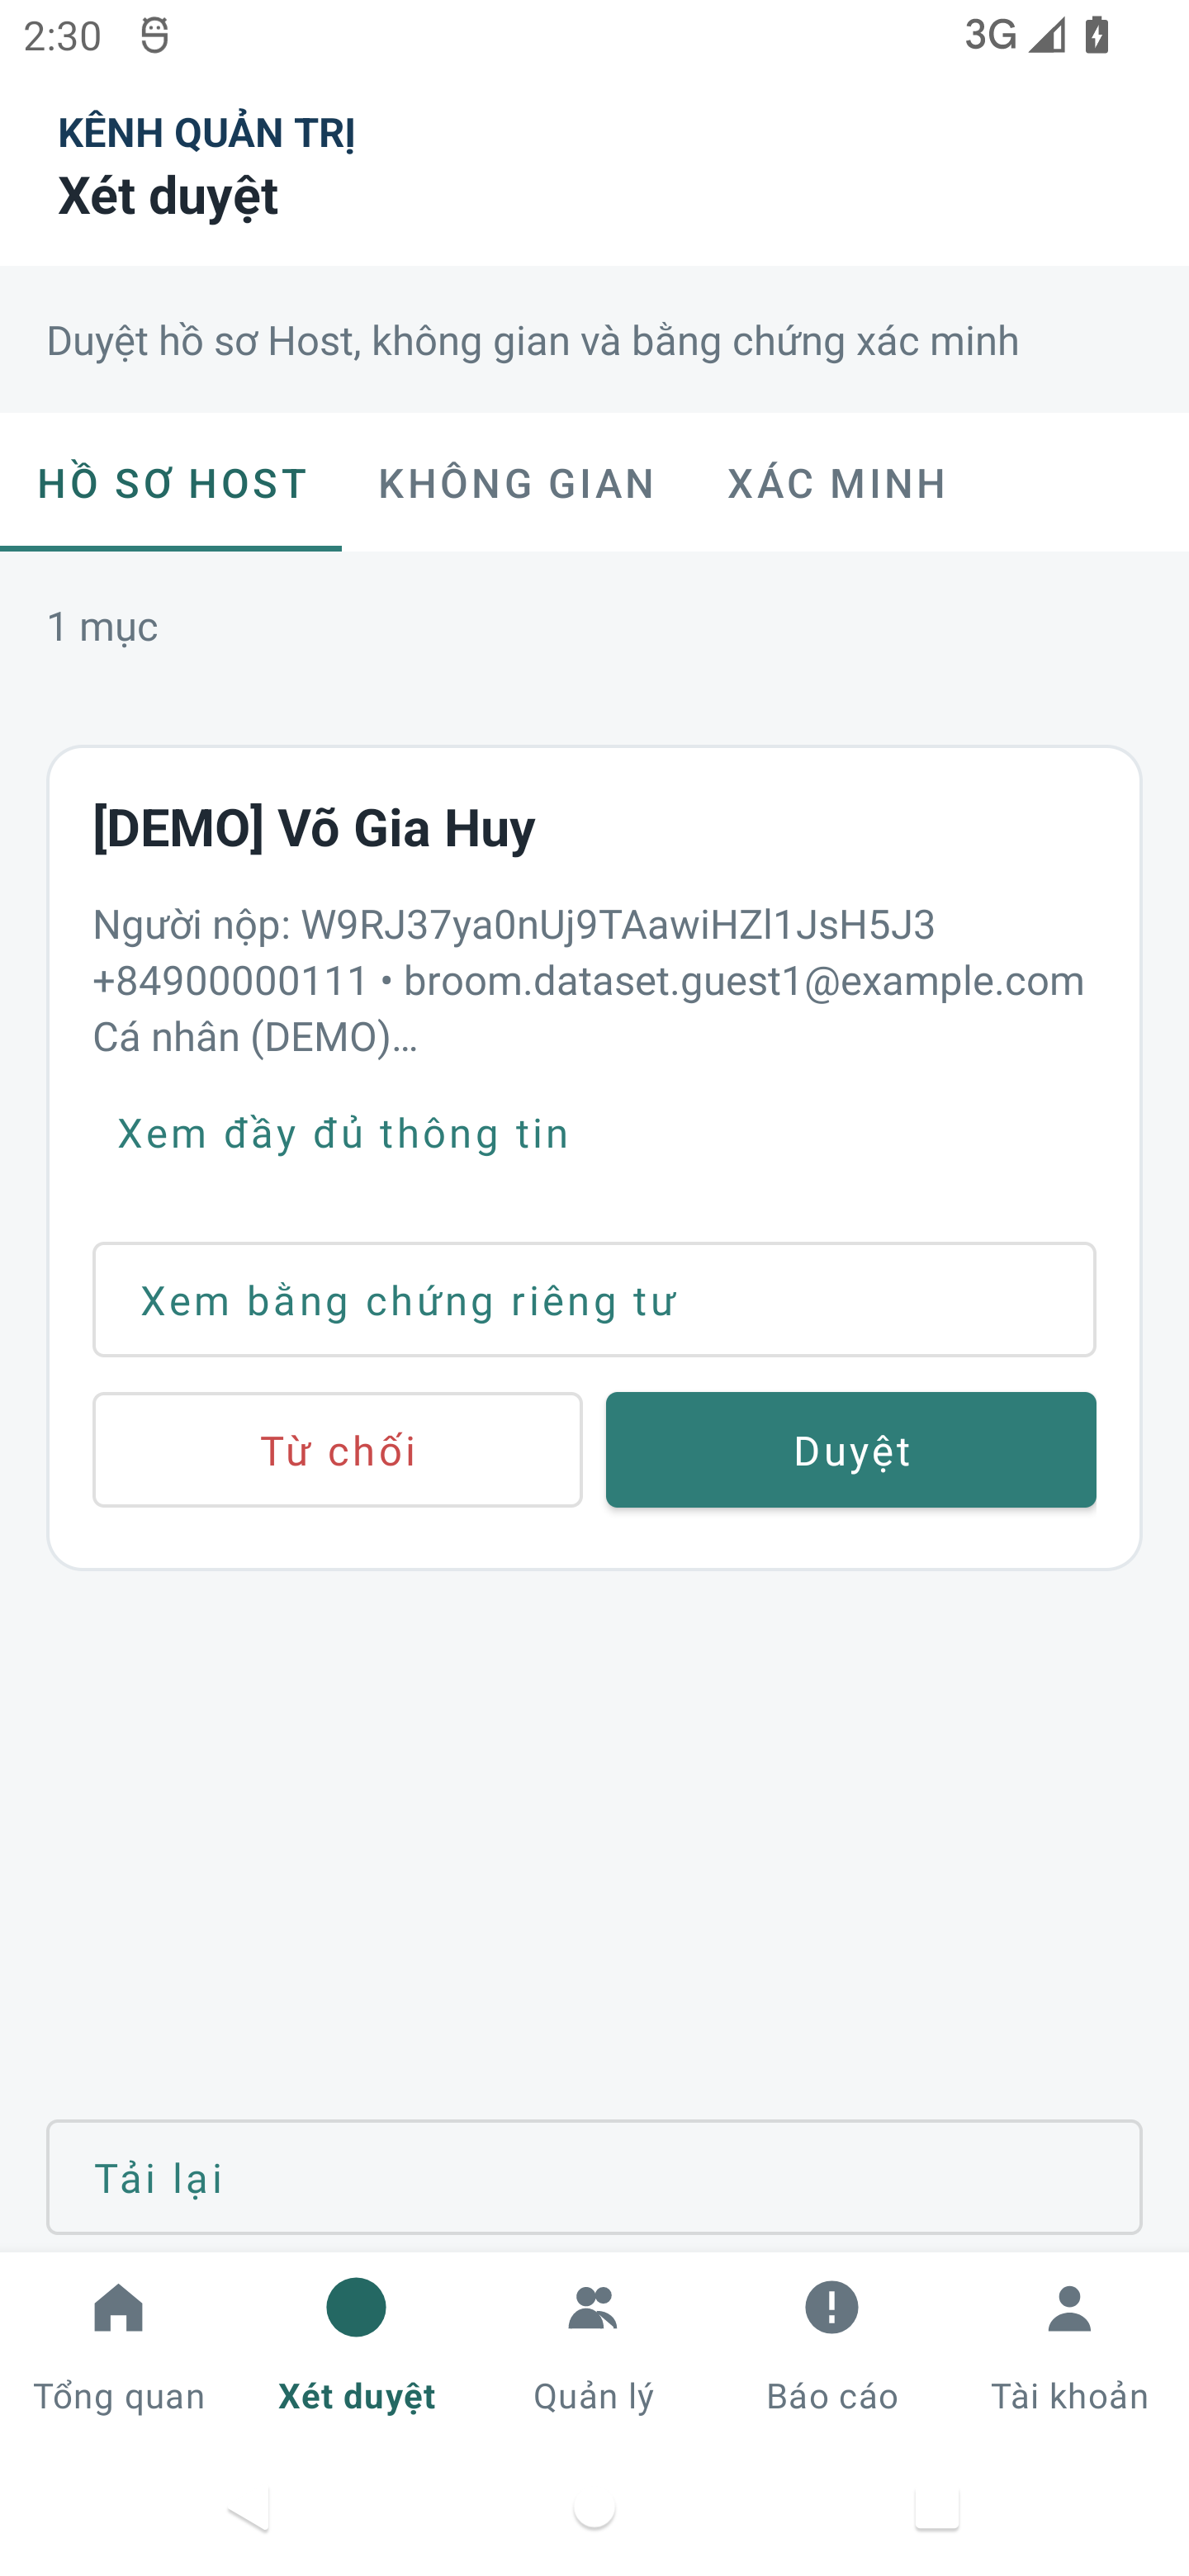
\includegraphics[width=\linewidth]{chapter5/admin-applications.png}\\[-1mm]
{\small (a) Hồ sơ xin quyền Host}
\end{minipage}\hspace{0.05\linewidth}%
\begin{minipage}[t]{0.40\linewidth}\centering
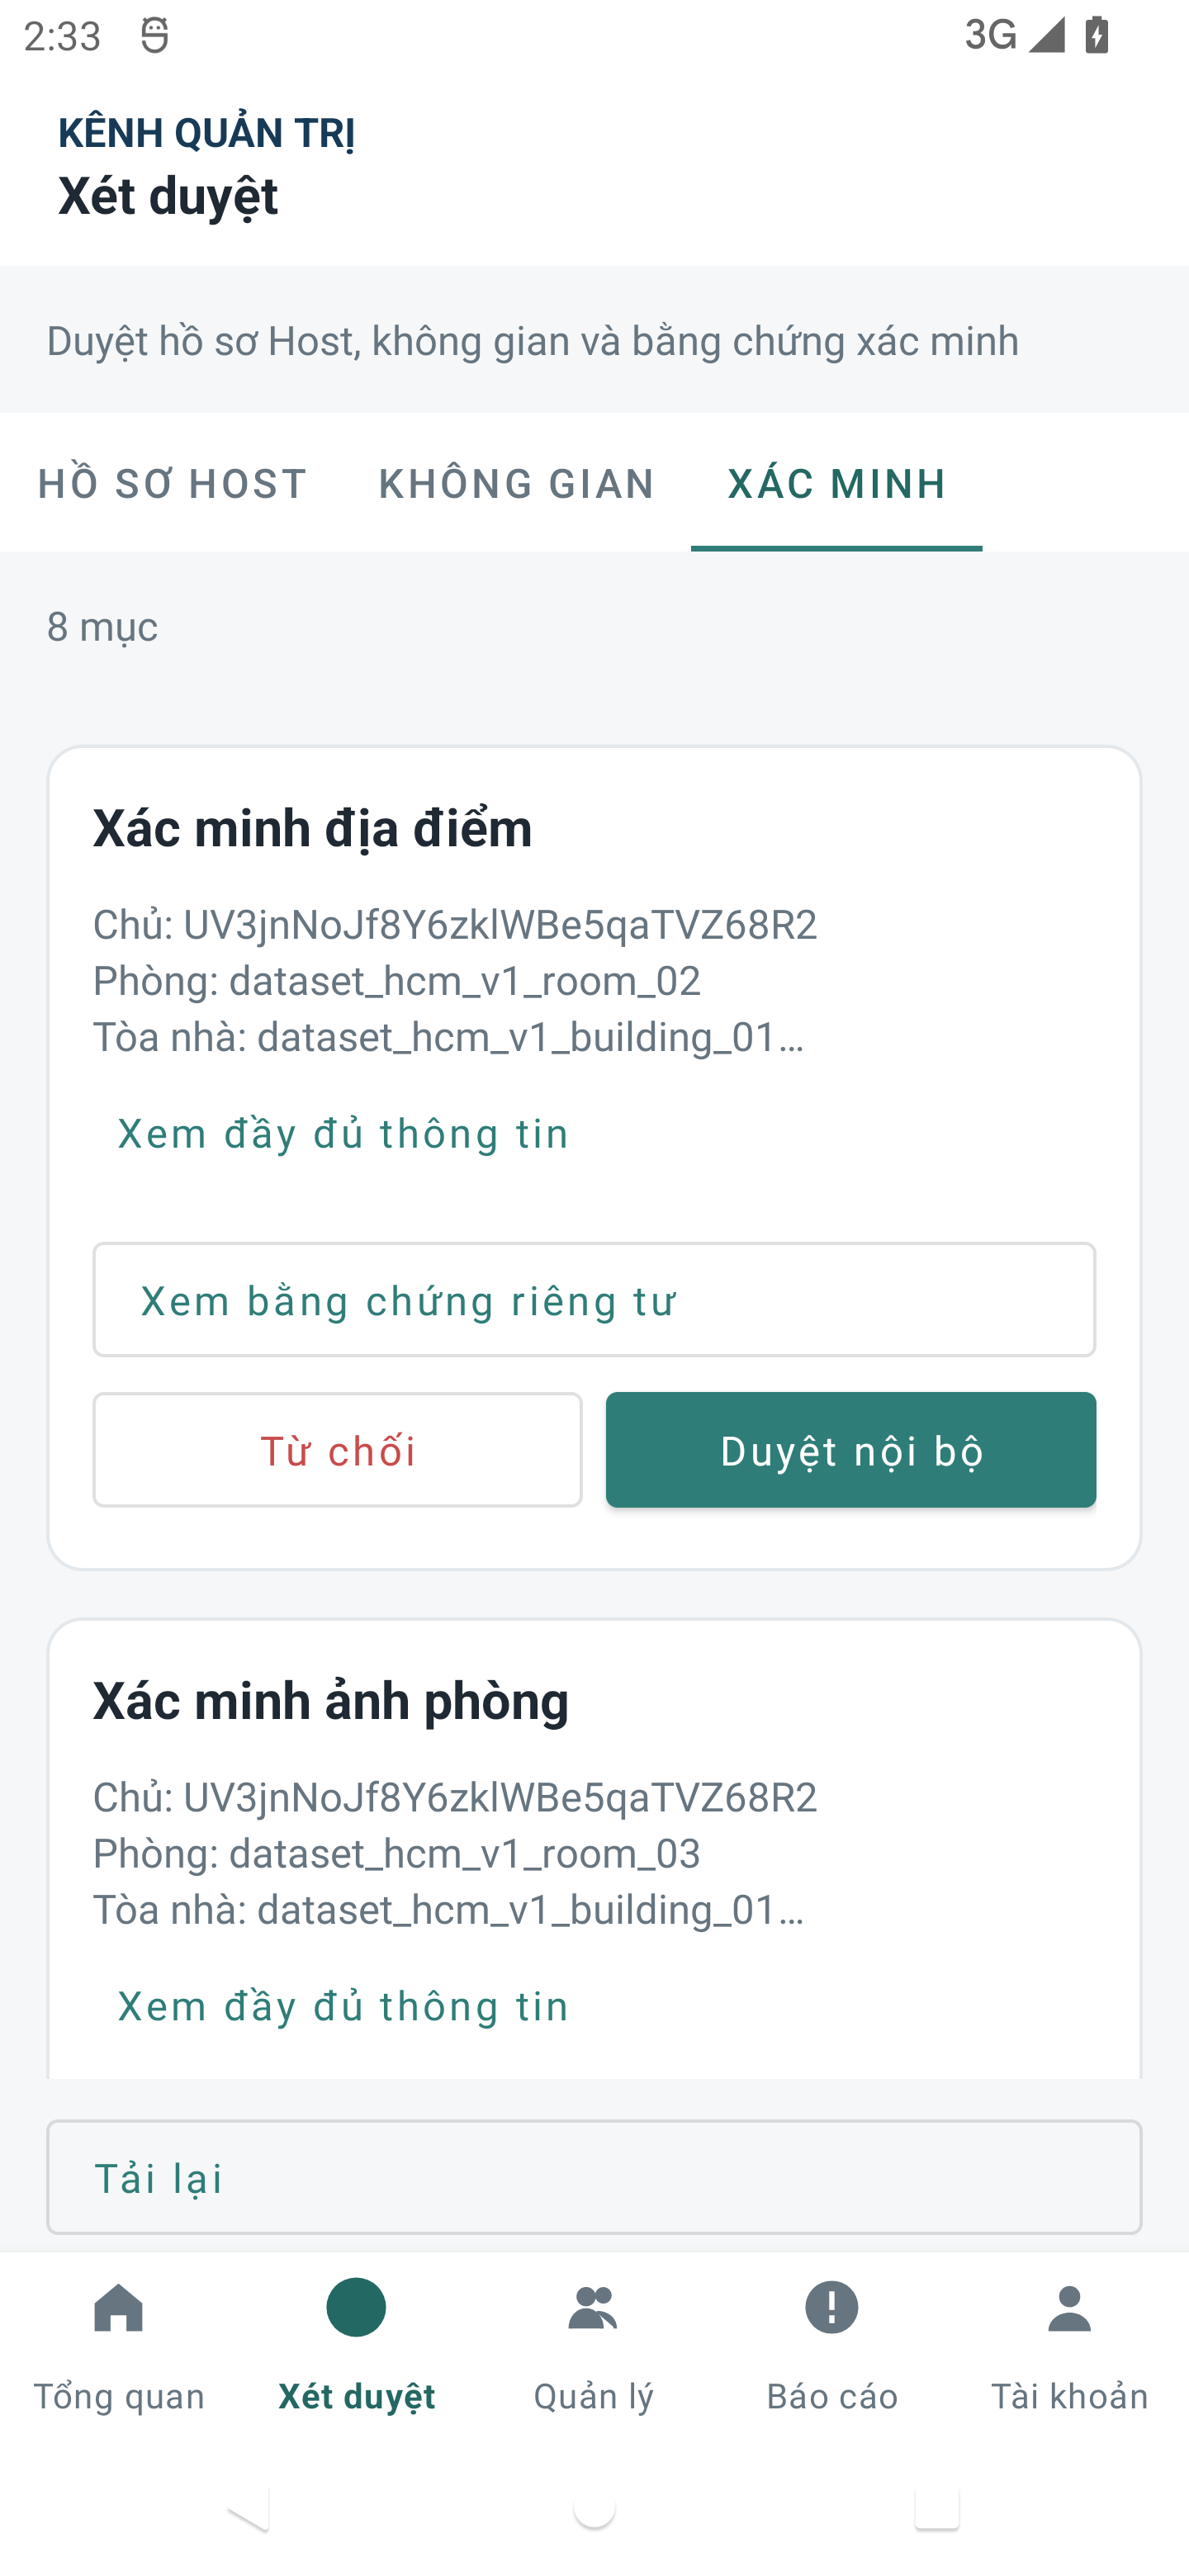
\includegraphics[width=\linewidth]{chapter5/admin-verifications.png}\\[-1mm]
{\small (b) Minh chứng vị trí và ảnh}
\end{minipage}
\caption{Hàng đợi hồ sơ Host và minh chứng không gian}
\label{fig:admin-application-evidence}
\end{figure}}{}

\IfFileExists{Resources/chapter5/admin-hosts.png}{%
Hình~\ref{fig:admin-host-audit}(a) hiển thị tài khoản Host cùng trạng thái hoạt động và thao tác khóa hoặc mở khóa tương ứng. Lý do xử lý được lưu để đối chiếu khi quản lý quyền nhận đặt mới. Nhật ký ở Hình~\ref{fig:admin-host-audit}(b) trình bày hành động, người thực hiện, đối tượng và thay đổi trạng thái theo thời gian. Admin có thể mở nội dung đầy đủ để kiểm tra một quyết định cụ thể; danh sách được giới hạn ở 100 thao tác mới nhất.
\begin{figure}[H]
\centering
\begin{minipage}[t]{0.40\linewidth}\centering
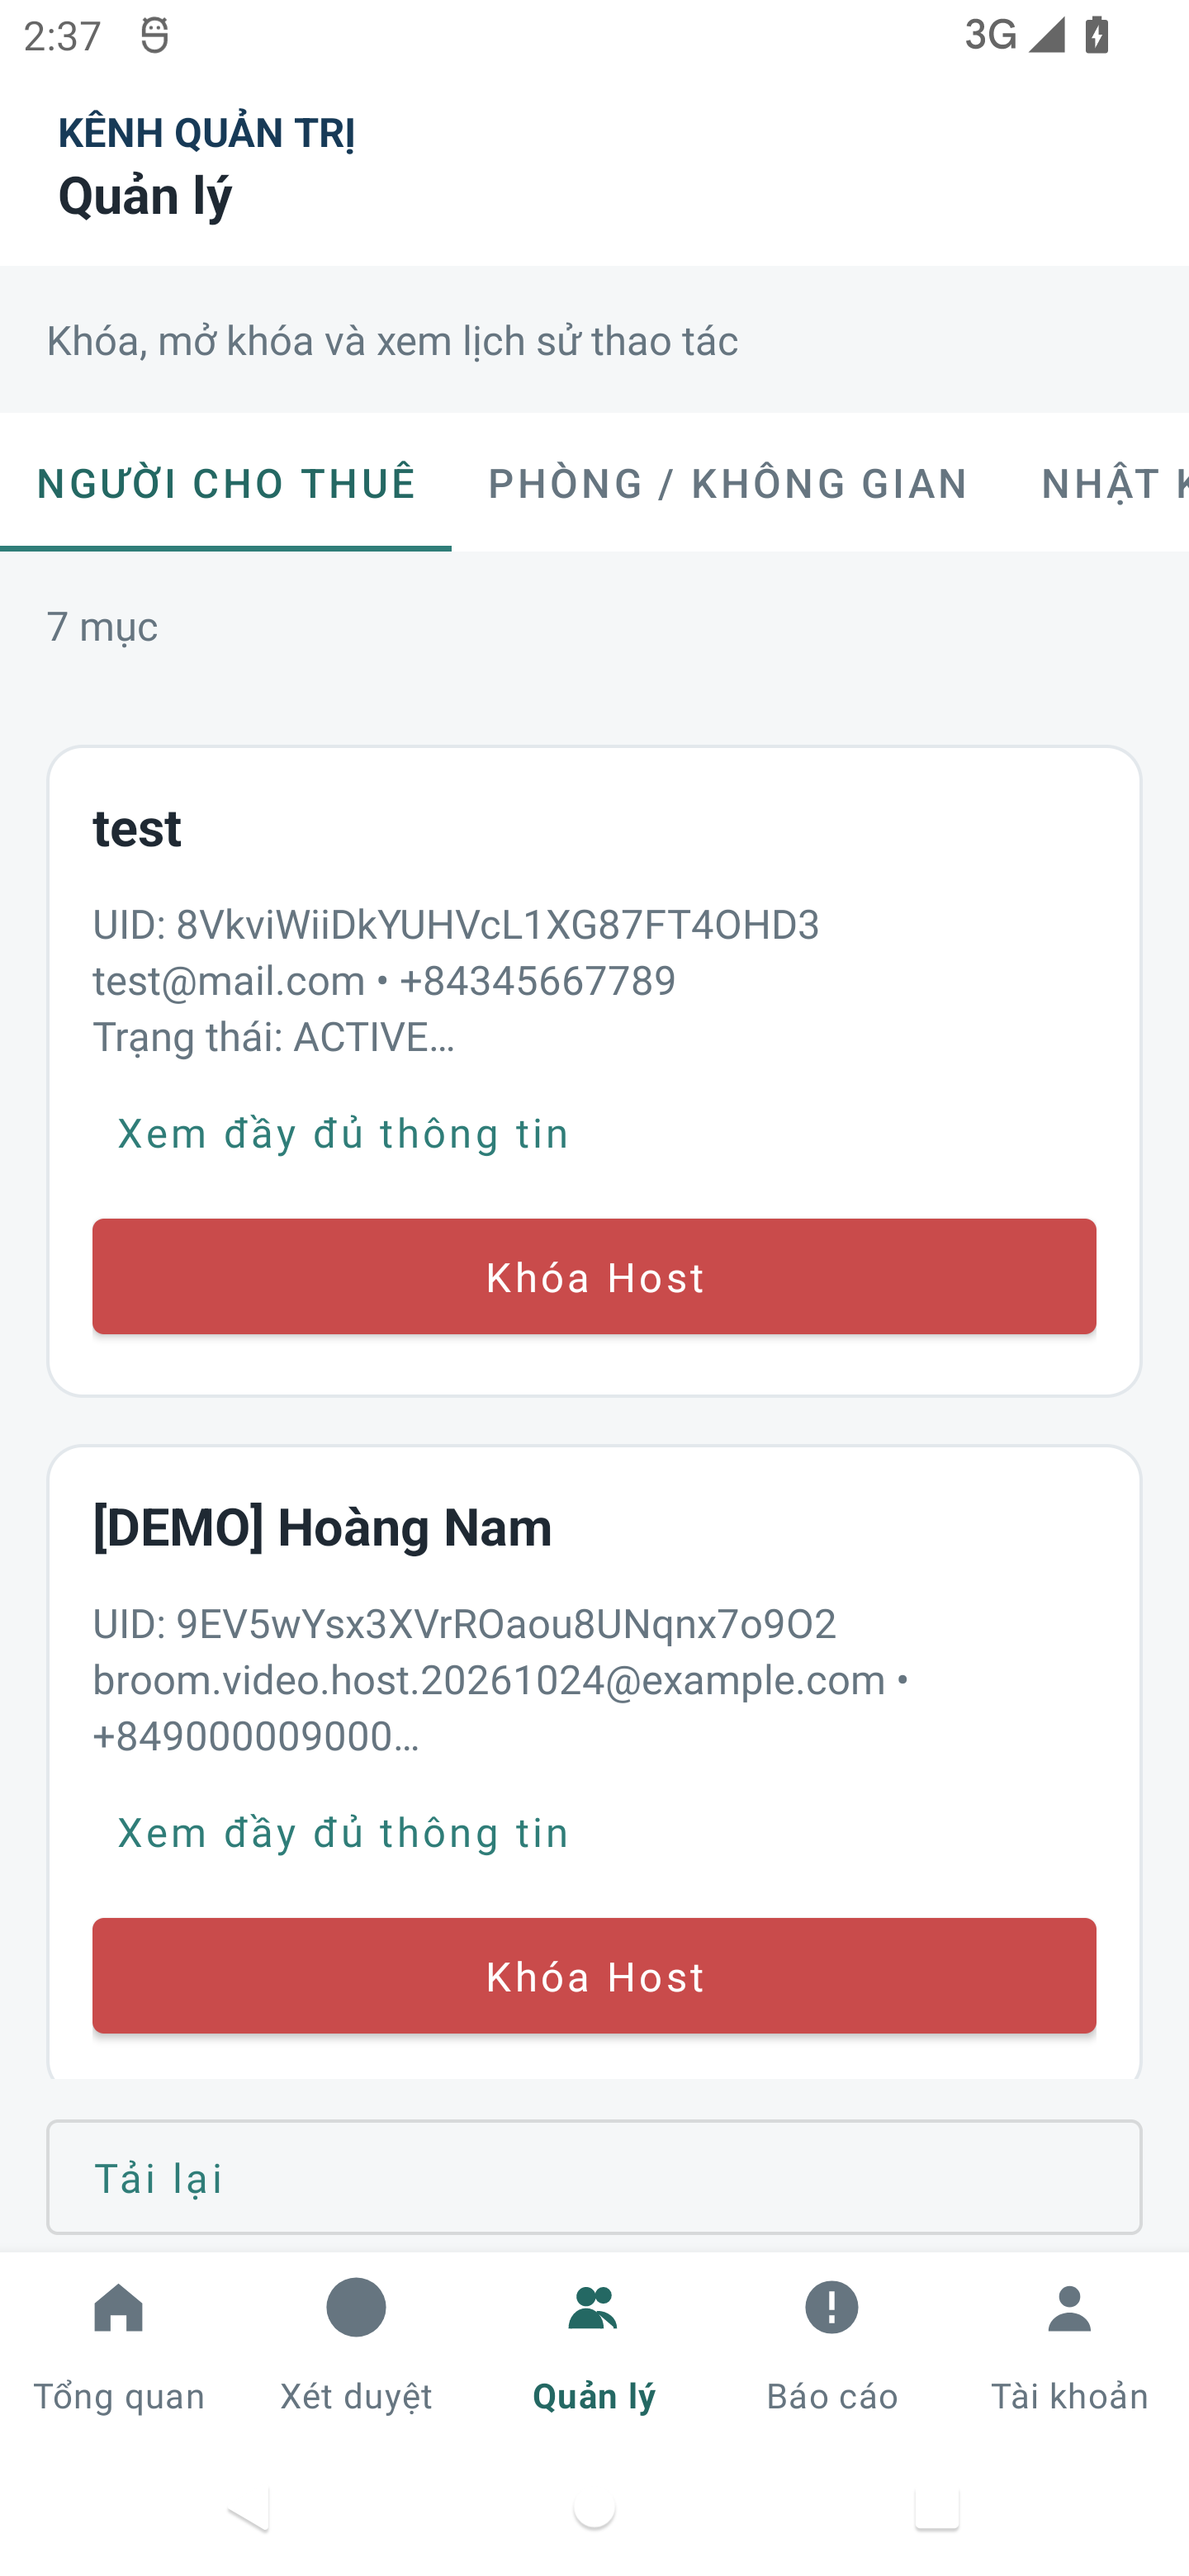
\includegraphics[width=\linewidth]{chapter5/admin-hosts.png}\\[-1mm]
{\small (a) Trạng thái Host}
\end{minipage}\hspace{0.05\linewidth}%
\begin{minipage}[t]{0.40\linewidth}\centering
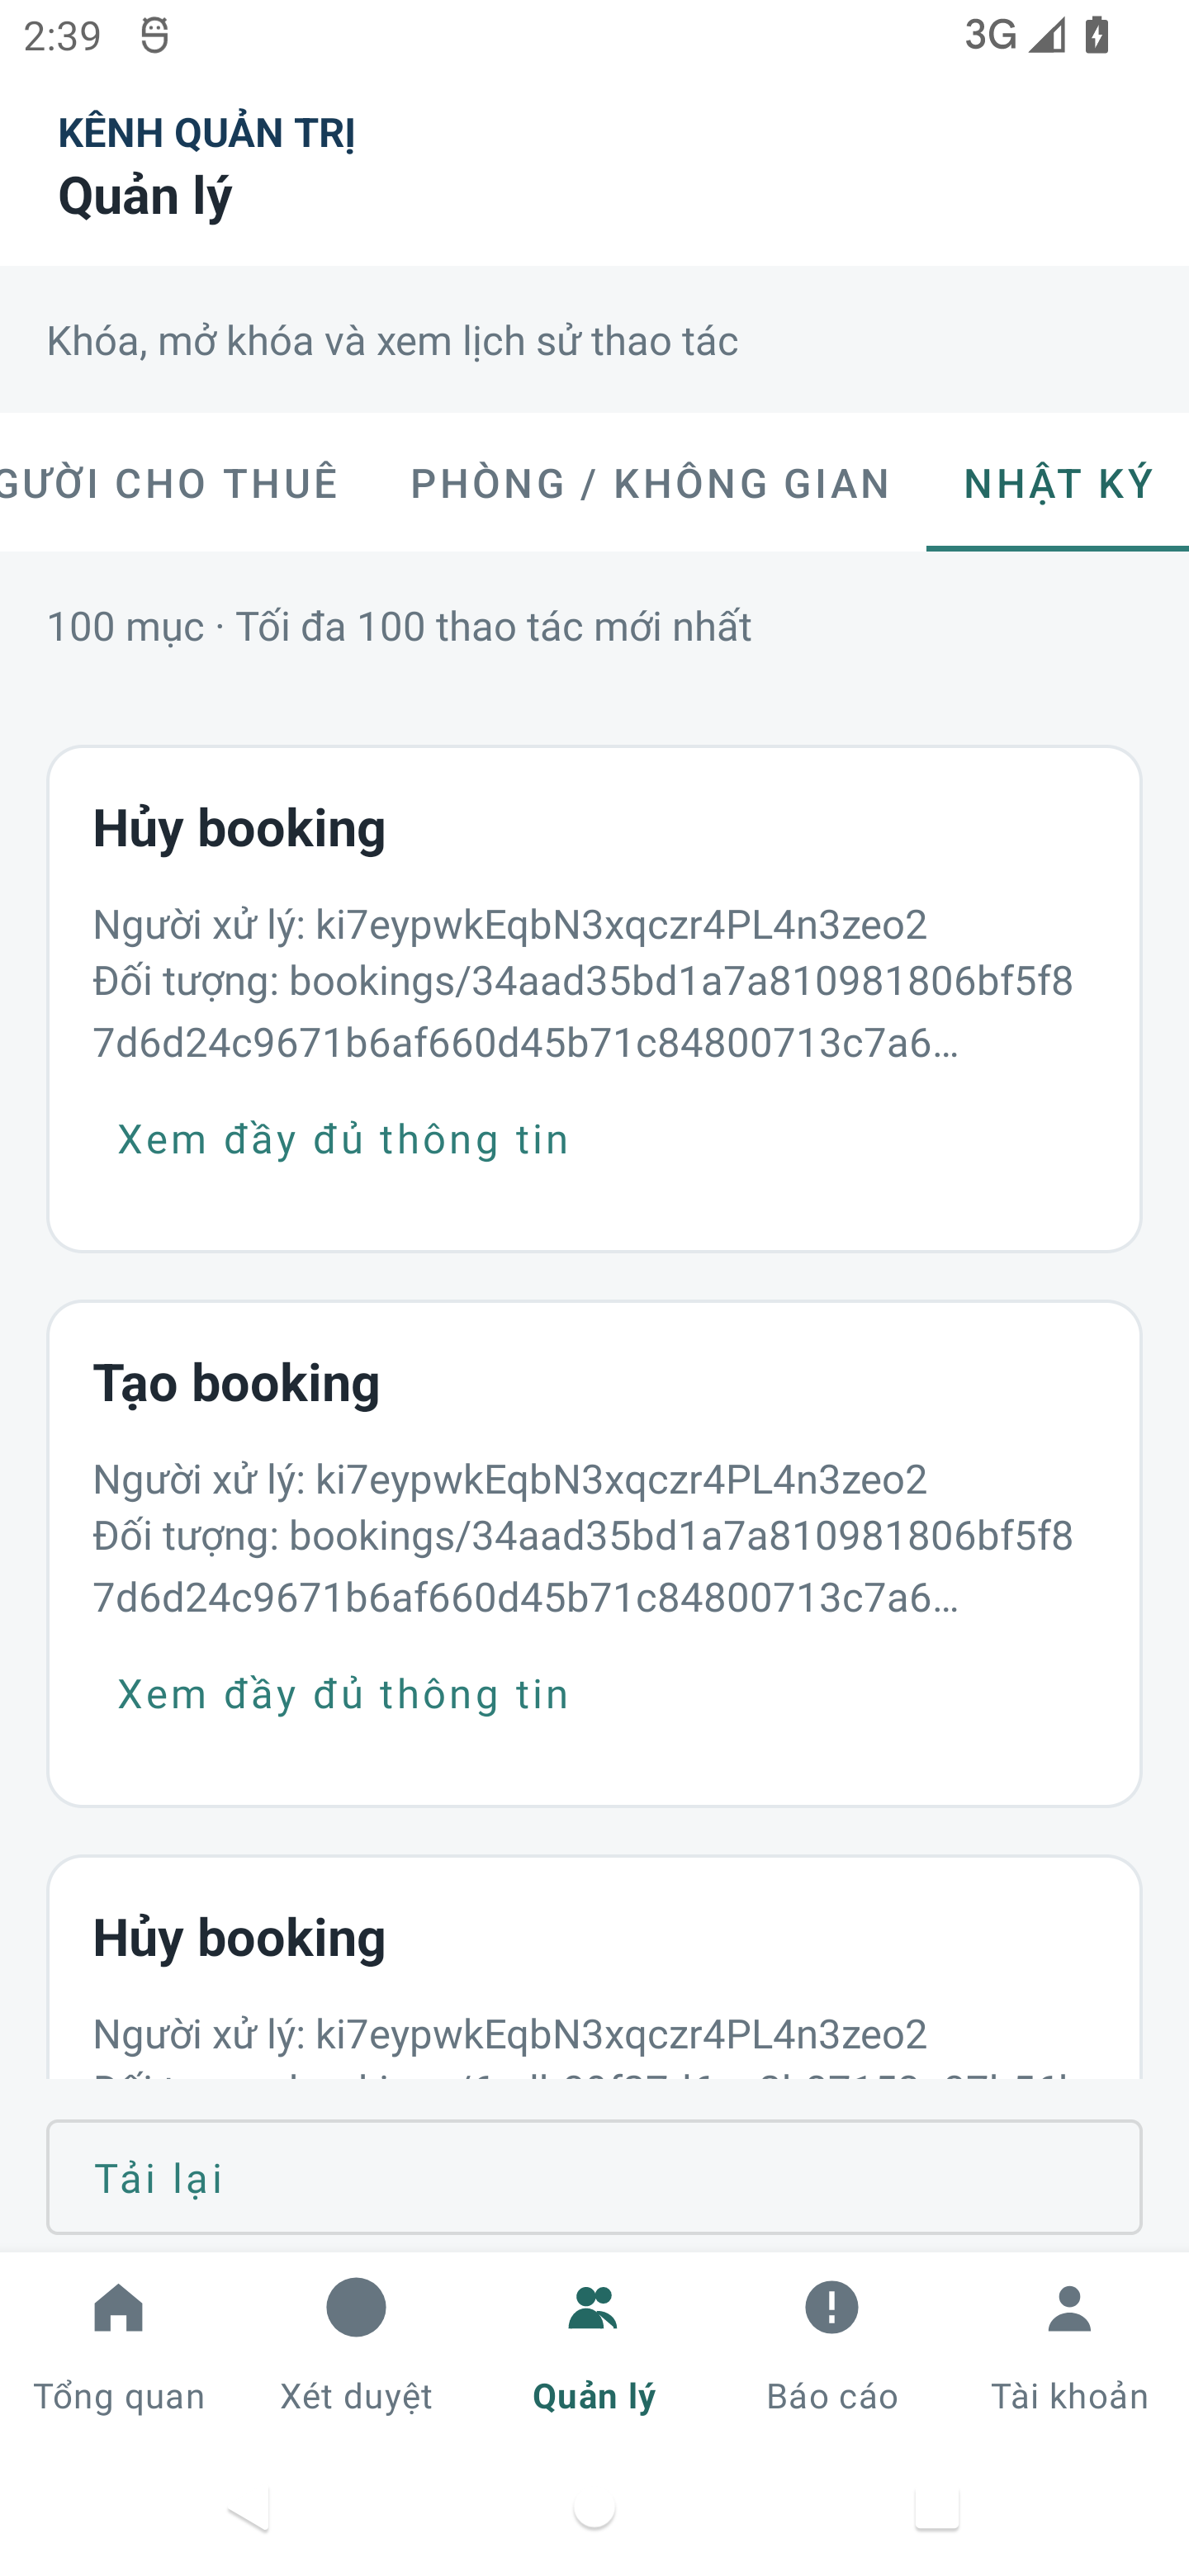
\includegraphics[width=\linewidth]{chapter5/admin-audit.png}\\[-1mm]
{\small (b) Nhật ký nghiệp vụ}
\end{minipage}
\caption{Giao diện quản lý Host và tra cứu nhật ký}
\label{fig:admin-host-audit}
\end{figure}}{}

